\chapter{Implementation}
\label{ch:implementation}

% Choose your own headings.

\section{System architecture}

During the development phase, several challenges were encountered, notably the difficulty in identifying a suitable nonprofit organization to receive donations. This obstacle has influenced the project's direction and necessitated adjustments to the original plan.

Given more time, I intend to reach out to local community members to establish a nonprofit organization dedicated to the cause, fostering greater local involvement and ensuring compliance with regional laws and regulations.

As a result, the donation page remains under development, as it requires collaboration with local nonprofits to provide accurate information on how to receive donations and adhere to legal requirements. This delay has impacted the project's timeline and scope.

To create a more comprehensive and impactful platform, the decision was made to incorporate a login page that offers educational resources on environmental conservation. This addition allows students and community members to engage with the content, learn about sustainable practices, and contribute to the preservation of the local environment. This enhancement not only enriches the project but also aligns with its broader goals of fostering environmental awareness and action.

The Farol de Santa Marta website is designed with two primary components: an API that connects to a database to store information about environmental conservation activities, events, courses, and products, and a web application that serves both the general public and organizers. Visitors interested in environmental conservation can explore information on upcoming events, educational courses, and eco-friendly products provided through the API. Organizers can register and manage their events, courses, and even products in the online store.

The user journey begins with the login process, as illustrated in Diagram 1 made using Mermaid.js\cite{mermaid}. If a user does not have an account, they have the option to sign up. Once registered, the user can log in and be directed to the Dashboard. From the Dashboard, users can navigate through various sections such as "Events," "Courses," "Store," and "Get Involved." 

In the "Events" section, users can browse upcoming environmental conservation events. If no events match the user's selected criteria, a pop-up notification will alert them. If relevant events are available, a list will be presented, allowing the user to click on any event for more detailed information through a modal window.

In the "Courses" section, users can explore educational content on environmental conservation. Similar to the events, users can view detailed course information and enroll in courses that interest them.

The "Store" section offers eco-friendly products, where users can browse items, view details, and make purchases to support conservation efforts. 

This structure ensures that both participants and organizers have a smooth, intuitive experience, enabling them to engage fully with the environmental initiatives and offerings of Farol de Santa Marta.

\begin{figure}
    \centering
    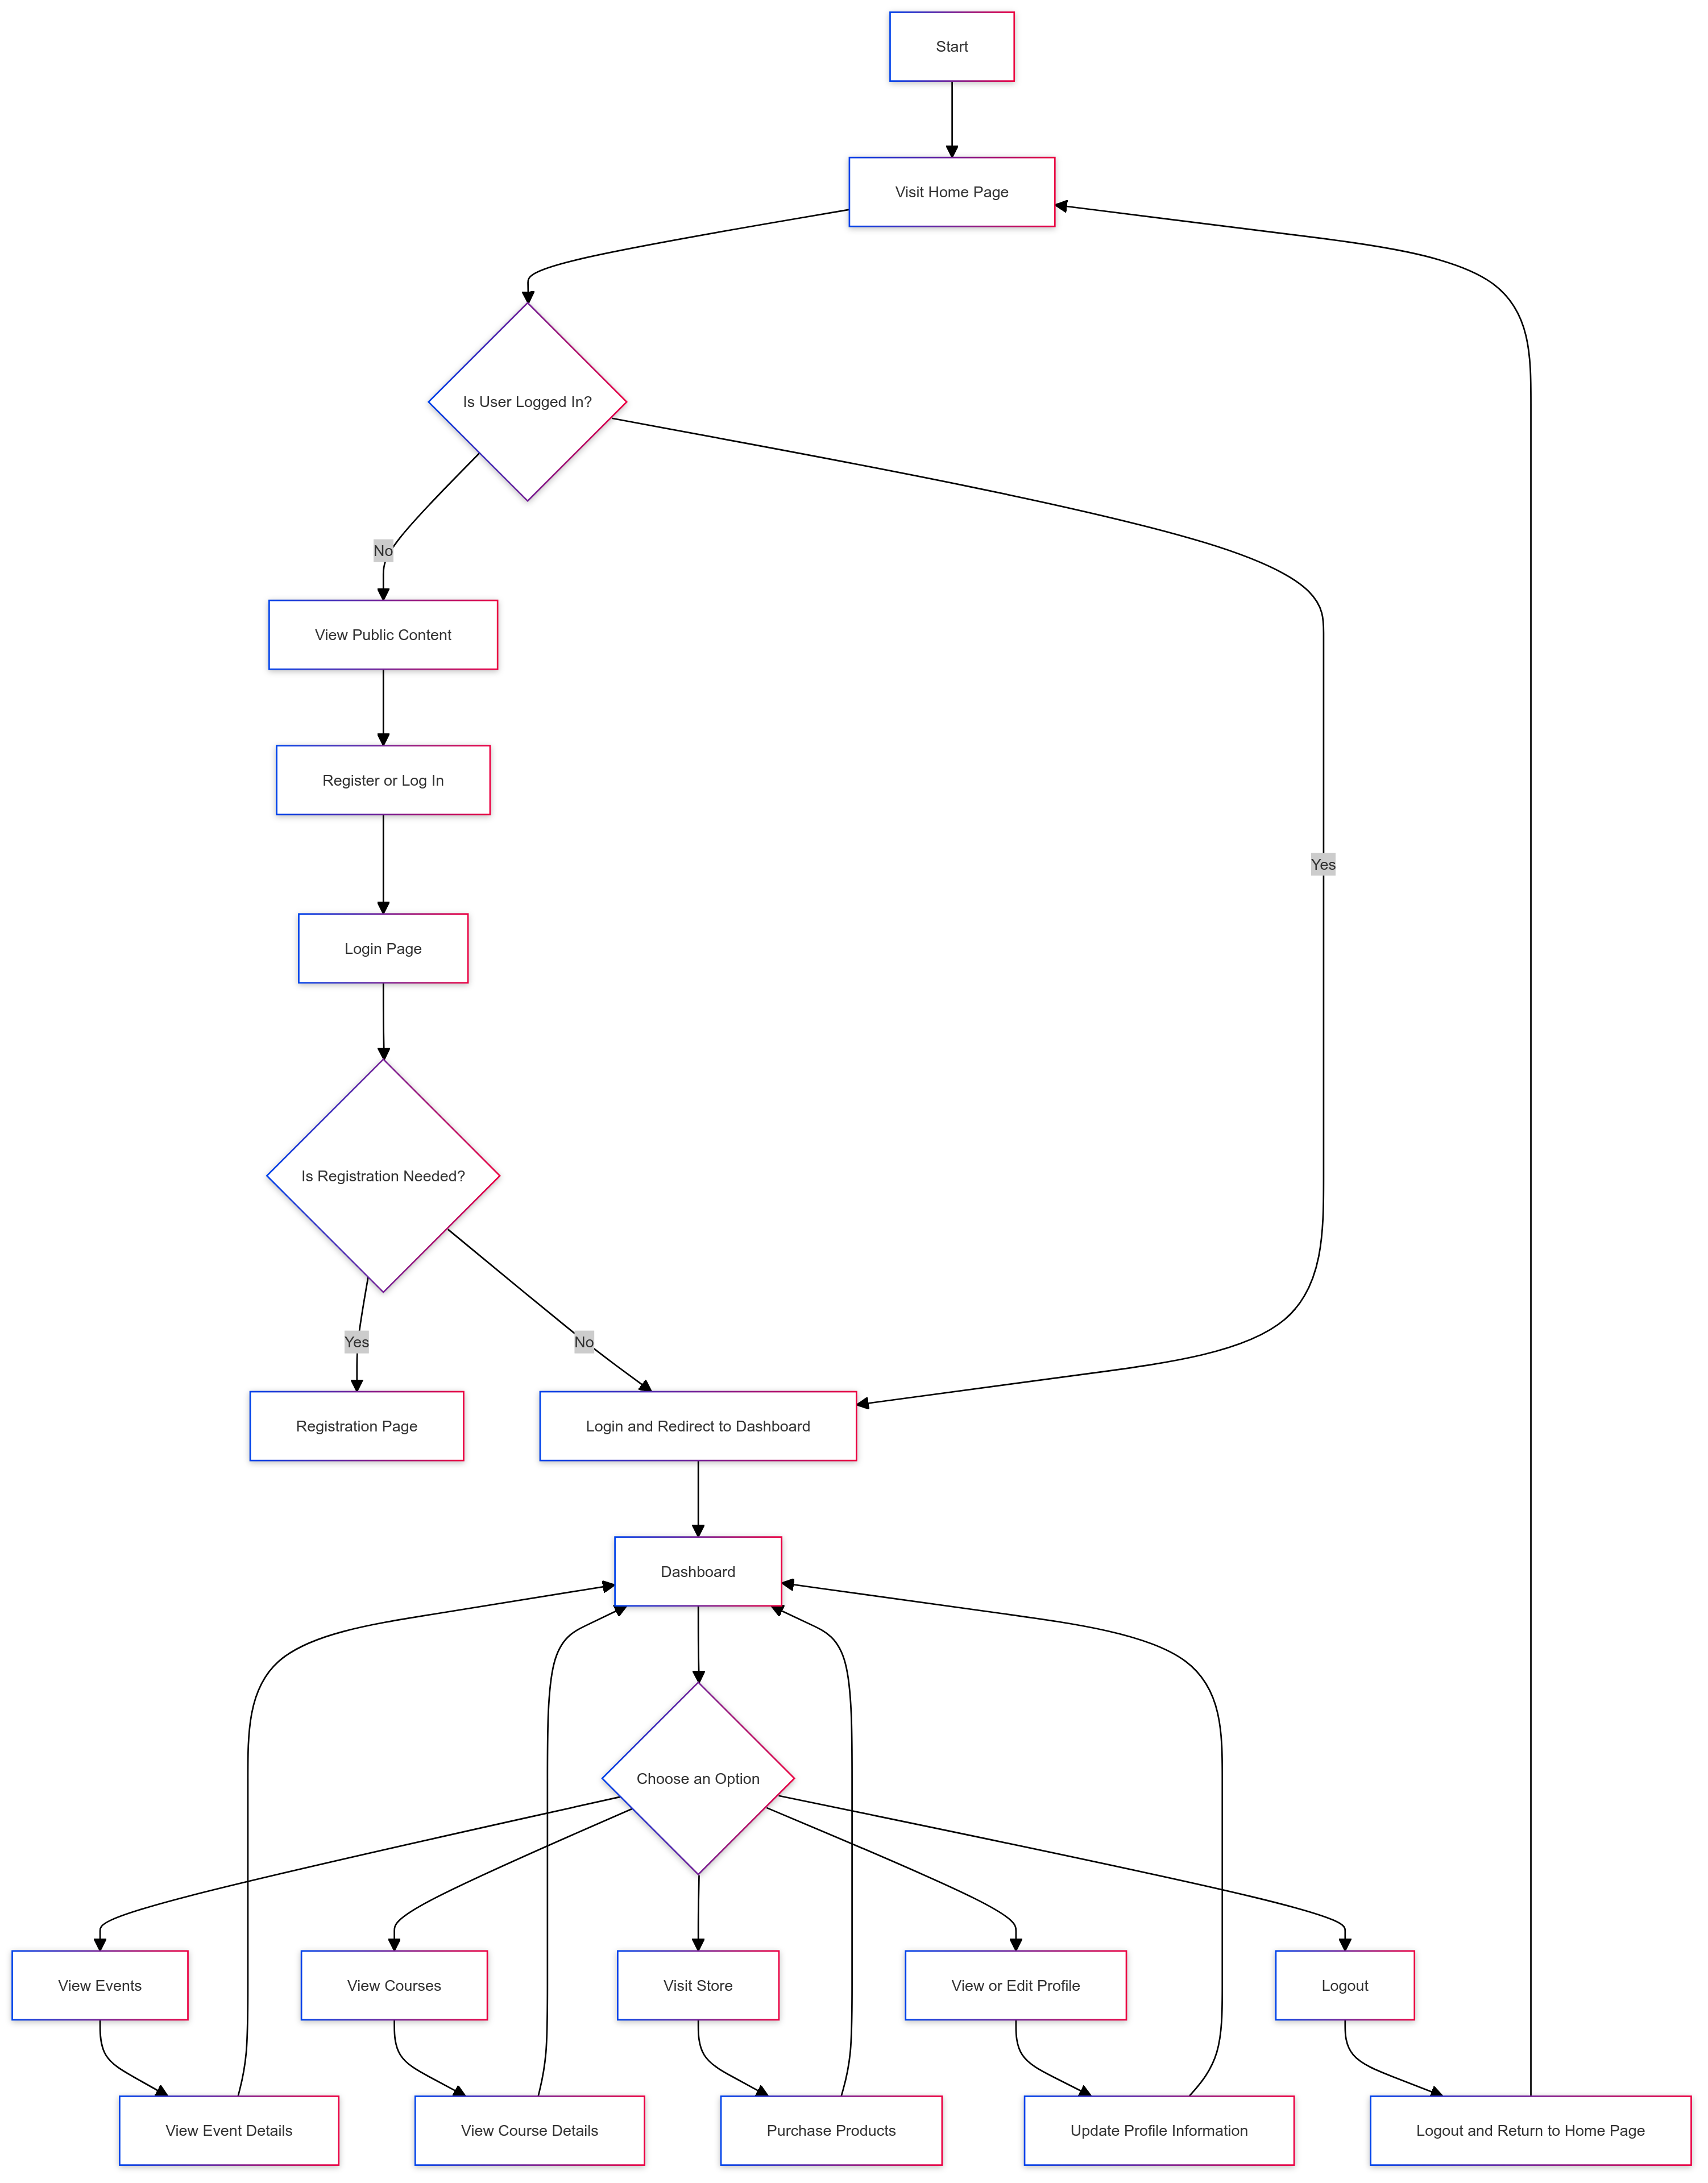
\includegraphics[width=1\linewidth]{images/mermaid-flow.png}
    \caption{Website Flowchart}
    \label{fig:Flowchart}
\end{figure}

\section{Software implementation}

The previous chapter presented the various technologies employed in the development of the Farol de Santa Marta website. This section delves deeper into the rationale behind the selection of these technologies and how each contributed to achieving the project’s goals.

Django, a high-level Python web framework, was chosen as the backbone of the website's backend. Its robust and scalable nature made it an ideal choice for managing the server-side logic of the application. Django’s built-in user authentication system allowed for secure user management, including login and registration functionalities. Furthermore, Django's ORM (Object-Relational Mapping) facilitated seamless interaction with the database, ensuring efficient data storage and retrieval operations.

SQLite was selected as the database solution for this project. As a lightweight, file-based database, SQLite was well-suited to the needs of this application, particularly given the project's scale. Its integration with Django is straightforward, allowing for quick setup and minimal configuration. SQLite's simplicity and reliability made it a fitting choice, ensuring that user data, events, courses, and other essential information could be managed efficiently.

On the front end, HTML5, CSS3, and JavaScript were used to structure, style, and add interactivity to the website. HTML5 provided a strong foundation for the markup, allowing for the creation of a semantically meaningful structure. CSS3 was utilized to ensure that the visual presentation of the website was both modern and responsive, making it accessible across various devices and screen sizes. JavaScript added the necessary interactivity, enabling dynamic user experiences that enhance engagement and usability.

Bootstrap was employed as the front-end framework to expedite the design process. Known for its responsive grid system and pre-built components, Bootstrap enabled the rapid development of a visually appealing and consistent user interface. This was particularly important for ensuring that the website could be accessed easily on different devices, providing a seamless experience whether users were on a desktop, tablet, or smartphone.

Mermaid.js was integrated into the project documentation to create diagrams and flowcharts that visually represent the system architecture and user navigation flows. This tool proved invaluable for communicating complex structures and processes clearly, making it easier for developers and stakeholders to understand the website’s design and functionality.

Finally, although still under development, the donation page will incorporate Stripe or a similar payment gateway. This technology was chosen for its reputation in handling secure online transactions, which is crucial for processing donations. Stripe's robust API and compliance with global financial regulations make it a reliable choice for ensuring that all transactions are processed securely and in accordance with legal requirements.

\section*{Intended Users}

The Farol de Santa Marta website is designed to serve a diverse audience, each with specific needs and motivations related to environmental conservation.

The primary user group consists of \textbf{local community members}, who are residents of Farol de Santa Marta and surrounding areas. These users are deeply invested in preserving their local environment and will utilize the website to stay informed about upcoming conservation events, participate in activities such as beach clean-ups, and access educational resources. Their primary motivation is to contribute to the preservation of their home, ensuring that the natural beauty of Farol de Santa Marta is maintained for future generations.

Another significant user group includes \textbf{tourists}, both domestic and international, who visit the region to enjoy its scenic beaches and natural attractions. These users seek information on local conservation practices and opportunities to engage in eco-friendly activities during their stay. They are motivated by a desire to enjoy the natural beauty of the area while minimizing their environmental impact, in line with the growing trend of sustainable tourism.

\textbf{Environmental activists and volunteers} also represent a key demographic for the website. These individuals are passionate about conservation and may or may not be local to the area. They will use the platform to find volunteer opportunities, make donations, and connect with like-minded individuals and organizations. Their motivation is driven by a strong commitment to sustainability and the desire to take actionable steps to protect the environment.

The website also targets \textbf{students and educators} interested in environmental studies, particularly those focused on marine and coastal ecosystems. Students will use the platform to enroll in educational courses, while educators may contribute content or use the site as a teaching tool. Their motivation lies in gaining and imparting knowledge about environmental conservation, with a focus on practical, community-based approaches.

Additionally, the website is intended for \textbf{nonprofit organizations and partners} involved in or supporting conservation efforts in the region. These organizations will use the platform to collaborate on projects, promote events, and connect with volunteers and donors. Their motivation is to expand their impact by engaging with a broader audience and securing resources for their initiatives.

\textbf{Donors}, who are individuals and entities interested in financially supporting environmental conservation in Farol de Santa Marta, will also find the website useful. They seek transparency regarding the use of their contributions and the impact of their donations. Their motivation is to support environmental causes and ensure that their financial contributions are making a tangible difference.

Finally, the website will be managed by \textbf{website administrators}, who are responsible for maintaining and updating the site. These users need tools to efficiently manage content, user roles, and technical operations, ensuring the website's smooth operation and its ability to meet the needs of its diverse user base.

\newpage
\section*{Functional Requirements for the Farol de Santa Marta App}

\begin{longtable}{|>{\raggedright}m{2cm}|>{\raggedright}m{4cm}|>{\raggedright\arraybackslash}m{8cm}|}
\hline
\textbf{Identifier} & \textbf{Functional Requirement} & \textbf{Detailed Description} \\
\hline
RF-01 & User Registration & The user must have the ability to register in the system by providing information such as name, email, and password. \\
\hline
RF-02 & User Authentication & The user must have the ability to log in to the system using their credentials. \\
\hline
RF-03 & Course Enrollment & The student user must have the ability to enroll in environmental conservation courses available on the platform. \\
\hline
RF-04 & Course Creation & The teacher user must have the ability to create and manage courses, including adding descriptions and course materials. \\
\hline
RF-05 & Course Viewing & The user must have the ability to view a list of available courses and their details. \\
\hline
RF-06 & Course Feedback & The user must have the ability to leave feedback on courses they have participated in, including comments and ratings. \\
\hline
RF-07 & Product Purchase & The user must have the ability to purchase eco-friendly products from the platform's store. \\
\hline
RF-08 & Donations & The user must have the ability to make donations to support environmental conservation projects through the system. \\
\hline
RF-09 & Event Viewing & The user must have the ability to view environmental conservation events organized in the region. \\
\hline
RF-10 & User Logout & The user must have the ability to log out of the system to end their session. \\
\hline
\end{longtable}

\subsection*{Explanation of the Columns}

\begin{itemize}
    \item \textbf{Identifier}: The unique code assigned to each functional requirement.
    \item \textbf{Functional Requirement}: The name or title of the requirement.
    \item \textbf{Detailed Description}: A detailed explanation of what the functional requirement should accomplish within the system.
\end{itemize}

This table of functional requirements serves as a guide for development, ensuring that all key functionalities of the \textbf{Farol de Santa Marta App} are implemented as planned.

\section{Data Model and Attributes}

This section presents the data model used for the \textit{Farol de Santa Marta} application. The model is represented by an Entity-Relationship Diagram (ERD) that defines the entities, their attributes, and the relationships between them.

\subsection{Entities and Attributes}

The application model and attributes are described as the Figure shows:
\begin{figure}
    \centering
    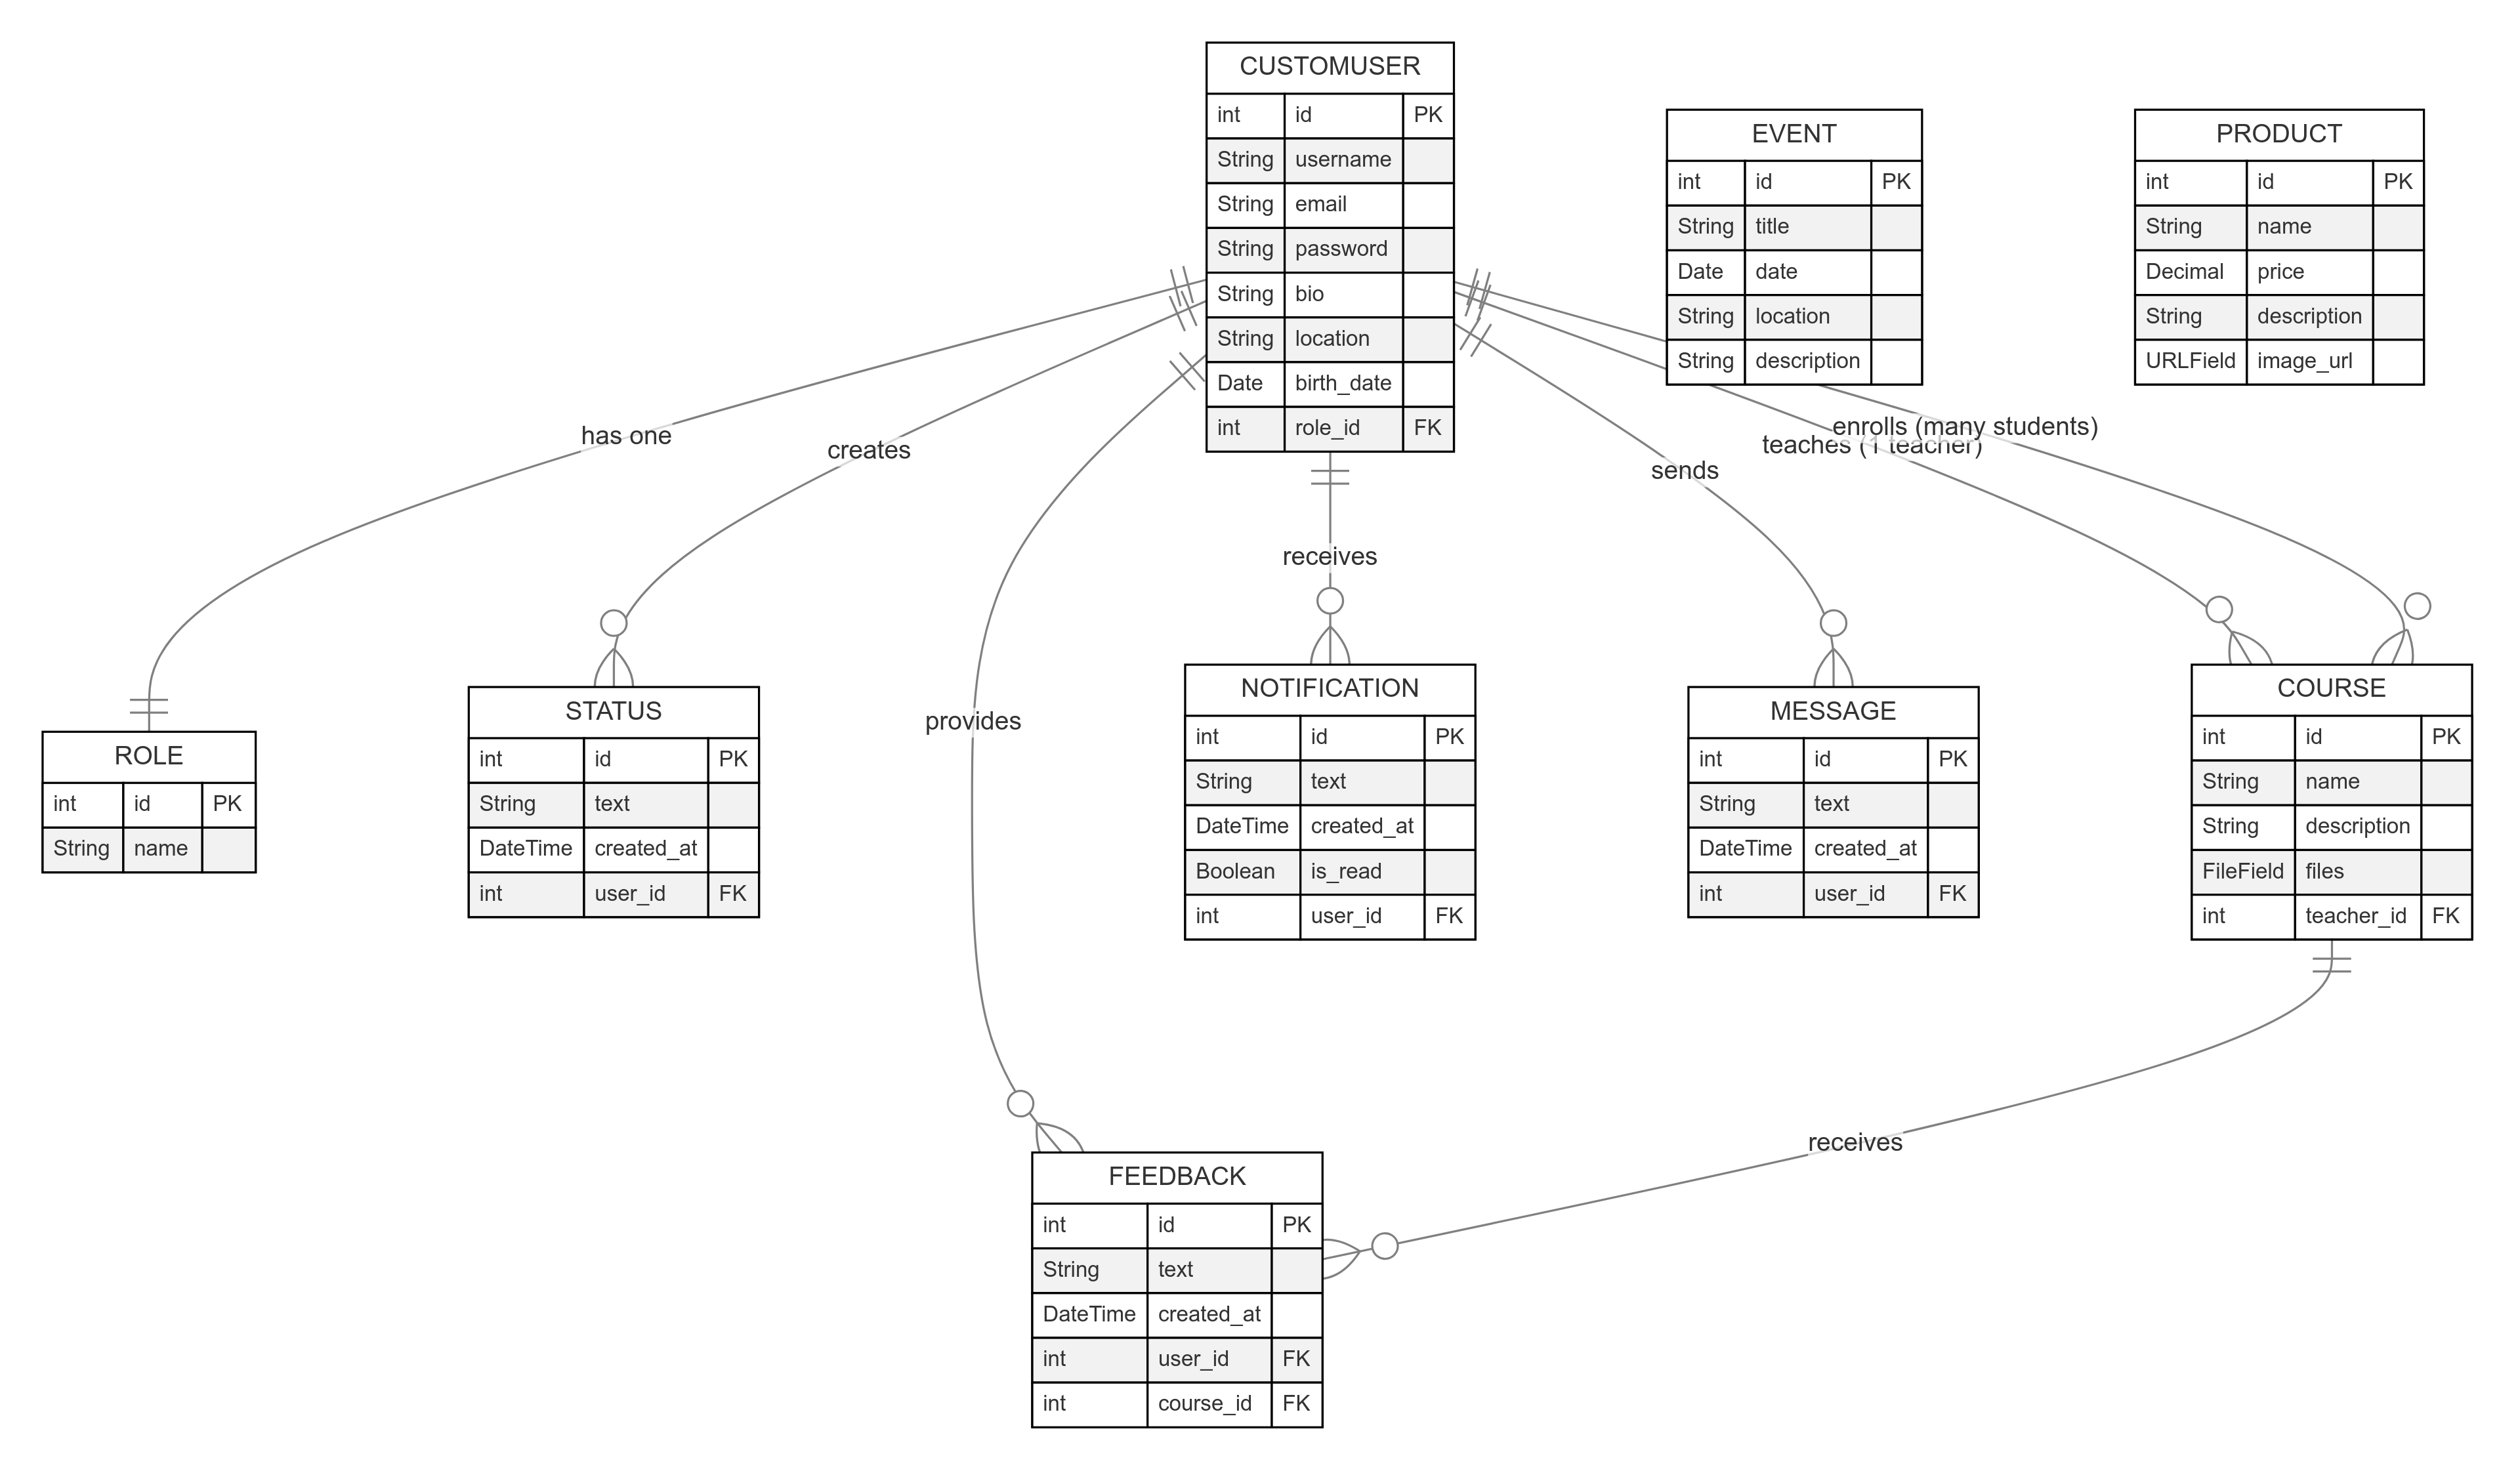
\includegraphics[width=1\linewidth]{images/er-diagram.png}
    \caption{ER Diagram}
    \label{fig:ER Diagram}
\end{figure}

\begin{itemize}
    \item \textbf{CUSTOMUSER}: The \texttt{CUSTOMUSER} entity represents the users of the system. Each user has the following attributes:
    \begin{itemize}
        \item \textbf{id (PK)}: A unique identifier for each user (Primary Key).
        \item \textbf{username}: The user's chosen name for logging into the system.
        \item \textbf{email}: The user's email address, used for communication and login purposes.
        \item \textbf{password}: The encrypted password for the user’s account.
        \item \textbf{bio}: A brief biography or description provided by the user.
        \item \textbf{location}: The user's location, which can be a city, state, or country.
        \item \textbf{birth\_date}: The user's birth date.
        \item \textbf{role\_id (FK)}: A foreign key linking the user to a specific role, enforcing the rule that each user can have only one role.
    \end{itemize}

    \item \textbf{ROLE}: The \texttt{ROLE} entity defines the different roles a user can have in the system. Each role has:
    \begin{itemize}
        \item \textbf{id (PK)}: A unique identifier for each role (Primary Key).
        \item \textbf{name}: The name of the role (e.g., "Student", "Teacher").
    \end{itemize}

    \item \textbf{STATUS}: The \texttt{STATUS} entity represents status updates posted by users. Attributes include:
    \begin{itemize}
        \item \textbf{id (PK)}: A unique identifier for each status update (Primary Key).
        \item \textbf{text}: The content of the status update.
        \item \textbf{created\_at}: The timestamp of when the status was created.
        \item \textbf{user\_id (FK)}: A foreign key linking the status to a specific user.
    \end{itemize}

    \item \textbf{COURSE}: The \texttt{COURSE} entity represents the courses offered in the system. Each course has:
    \begin{itemize}
        \item \textbf{id (PK)}: A unique identifier for each course (Primary Key).
        \item \textbf{name}: The name of the course.
        \item \textbf{description}: A brief description of what the course entails.
        \item \textbf{files}: A field for uploading course-related files (e.g., PDFs, documents).
        \item \textbf{teacher\_id (FK)}: A foreign key linking the course to the teacher who created it.
    \end{itemize}

    \item \textbf{FEEDBACK}: The \texttt{FEEDBACK} entity captures feedback provided by users on specific courses. Attributes include:
    \begin{itemize}
        \item \textbf{id (PK)}: A unique identifier for each feedback entry (Primary Key).
        \item \textbf{text}: The content of the feedback.
        \item \textbf{created\_at}: The timestamp of when the feedback was provided.
        \item \textbf{user\_id (FK)}: A foreign key linking the feedback to the user who provided it.
        \item \textbf{course\_id (FK)}: A foreign key linking the feedback to the specific course it relates to.
    \end{itemize}

    \item \textbf{NOTIFICATION}: The \texttt{NOTIFICATION} entity represents notifications sent to users. Each notification has:
    \begin{itemize}
        \item \textbf{id (PK)}: A unique identifier for each notification (Primary Key).
        \item \textbf{text}: The content of the notification.
        \item \textbf{created\_at}: The timestamp of when the notification was created.
        \item \textbf{is\_read}: A boolean value indicating whether the notification has been read.
        \item \textbf{user\_id (FK)}: A foreign key linking the notification to a specific user.
    \end{itemize}

    \item \textbf{MESSAGE}: The \texttt{MESSAGE} entity stores messages sent by users. Attributes include:
    \begin{itemize}
        \item \textbf{id (PK)}: A unique identifier for each message (Primary Key).
        \item \textbf{text}: The content of the message.
        \item \textbf{created\_at}: The timestamp of when the message was sent.
        \item \textbf{user\_id (FK)}: A foreign key linking the message to the user who sent it.
    \end{itemize}

    \item \textbf{EVENT}: The \texttt{EVENT} entity represents events related to environmental conservation activities. Each event has:
    \begin{itemize}
        \item \textbf{id (PK)}: A unique identifier for each event (Primary Key).
        \item \textbf{title}: The title or name of the event.
        \item \textbf{date}: The date when the event is scheduled to occur.
        \item \textbf{location}: The location where the event will take place.
        \item \textbf{description}: A detailed description of the event.
    \end{itemize}

    \item \textbf{PRODUCT}: The \texttt{PRODUCT} entity represents items available for purchase in the system’s store. Each product has:
    \begin{itemize}
        \item \textbf{id (PK)}: A unique identifier for each product (Primary Key).
        \item \textbf{name}: The name of the product.
        \item \textbf{price}: The cost of the product, represented as a decimal value.
        \item \textbf{description}: A detailed description of the product.
        \item \textbf{image\_url}: A URL linking to an image of the product.
    \end{itemize}
\end{itemize}

\subsection{Relationships Between Entities}

\begin{itemize}
    \item \textbf{CUSTOMUSER and ROLE}: The relationship between \texttt{CUSTOMUSER} and \texttt{ROLE} is one-to-one, meaning each user can only have one role at a time.

    \item \textbf{CUSTOMUSER and STATUS}: A one-to-many relationship, where a user can create multiple status updates.

    \item \textbf{CUSTOMUSER and NOTIFICATION}: A one-to-many relationship, where a user can receive multiple notifications.

    \item \textbf{CUSTOMUSER and MESSAGE}: A one-to-many relationship, where a user can send multiple messages.

    \item \textbf{CUSTOMUSER and FEEDBACK}: A one-to-many relationship, where a user can provide feedback for multiple courses.

    \item \textbf{COURSE and FEEDBACK}: A one-to-many relationship, where a course can receive multiple feedback entries.

    \item \textbf{CUSTOMUSER and COURSE}:
    \begin{itemize}
        \item \textbf{Teacher Relationship}: A one-to-many relationship, where a teacher can create and manage multiple courses.
        \item \textbf{Student Relationship}: A many-to-many relationship, where multiple students can enroll in multiple courses.
    \end{itemize}
\end{itemize}

\section{Prototyping}

The design of the \textit{Farol de Santa Marta} website was heavily inspired by the best practices and successful strategies observed during the research phase. The initial prototype was developed with a strong emphasis on usability, accessibility, and visual appeal, drawing from the elements that were identified as effective in engaging users and promoting environmental causes.

\subsection{Inspiration from Existing Websites}

During the research phase, several websites were analyzed to understand how they effectively communicate their missions, engage with their audience, and drive user actions such as donations, volunteer sign-ups, and participation in educational activities. Key websites that influenced the design include:

\begin{itemize}
    \item \textbf{Charity: Water}: Known for its clean, visually striking interface and impactful use of imagery, \textit{Charity: Water} provided inspiration for the visual design of the \textit{Farol de Santa Marta} website. The use of high-quality images, clear typography, and a straightforward layout were key elements adopted from this site.

    \item \textbf{World Wildlife Fund (WWF)}: The \textit{WWF} website's effective use of concise messaging and strategic placement of calls-to-action (CTAs) influenced the placement and design of similar elements on the \textit{Farol de Santa Marta} platform. The emphasis on highlighting the impact of user contributions through powerful visuals and succinct text was a direct inspiration for the prototype.

    \item \textbf{Greenpeace}: The \textit{Greenpeace} website's focus on activism and community engagement provided valuable insights into designing interactive elements, such as the "Get Involved" section, which encourages users to participate in local conservation activities. The prototype incorporated similar engagement strategies to foster a sense of community and collective responsibility among users.
\end{itemize}

\section{Overview of Key Pages}

This chapter presents the implemented and operational application, in accordance with the functional and non-functional requirements of the system. It provides a detailed overview of the development of each feature and component. The implementation will be showcased in desktop mode.

\subsection{Home page}

The homepage of the Farol de Santa Marta website serves as the central hub for users, offering a welcoming and visually appealing introduction to the platform. Designed with both aesthetics and functionality in mind, the homepage features a prominent hero section with a background image that captures the natural beauty of the coastline, immediately engaging visitors. The page is structured to provide easy navigation, with clear calls-to-action that guide users to key sections such as events, courses, and ways to get involved in environmental conservation efforts. By combining responsive design elements with compelling content, the homepage effectively communicates the mission of Farol de Santa Marta and invites users to explore and participate in the community's efforts to preserve the local environment.

\begin{figure}[H]
    \centering
    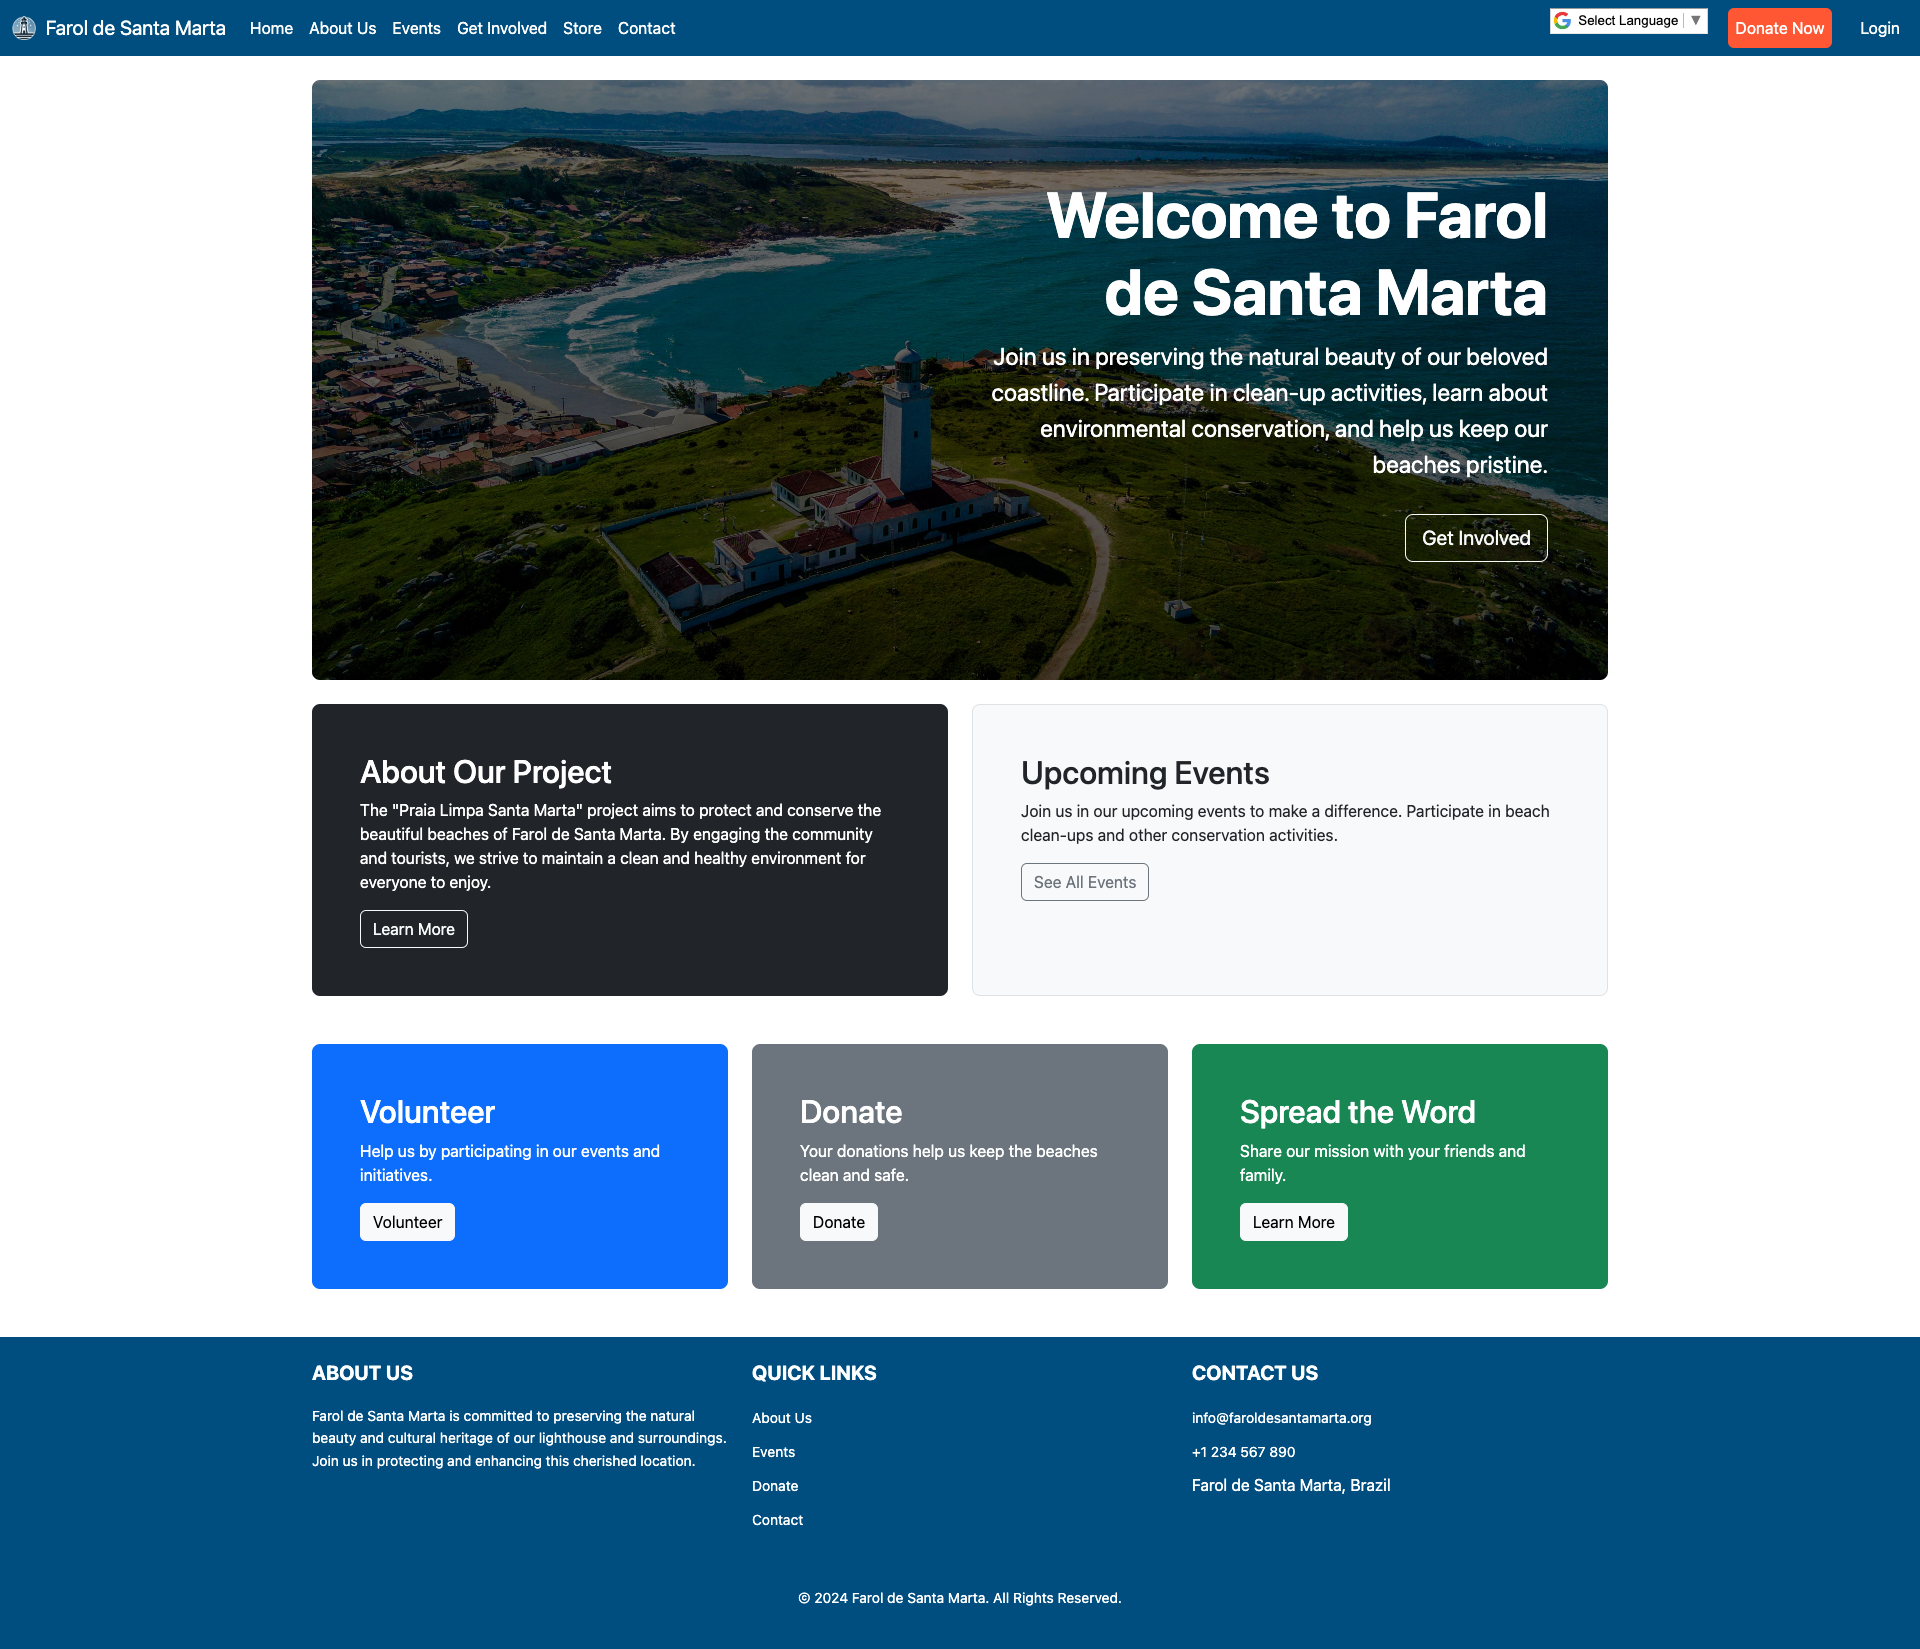
\includegraphics[width=1\linewidth]{images/home-page.png}
    \caption{Home page}
    \label{fig:Home page}
\end{figure}

\subsection{Events Page}

The \textbf{Events Page} serves as a central location for users to discover and participate in upcoming environmental conservation activities. It lists all the scheduled events, such as beach clean-ups and educational workshops, along with details including the date, location, and a brief description of each event. Users can easily browse through the events, click for more details, and sign up to participate, fostering community involvement in local conservation efforts.

\begin{figure}[H]
    \centering
    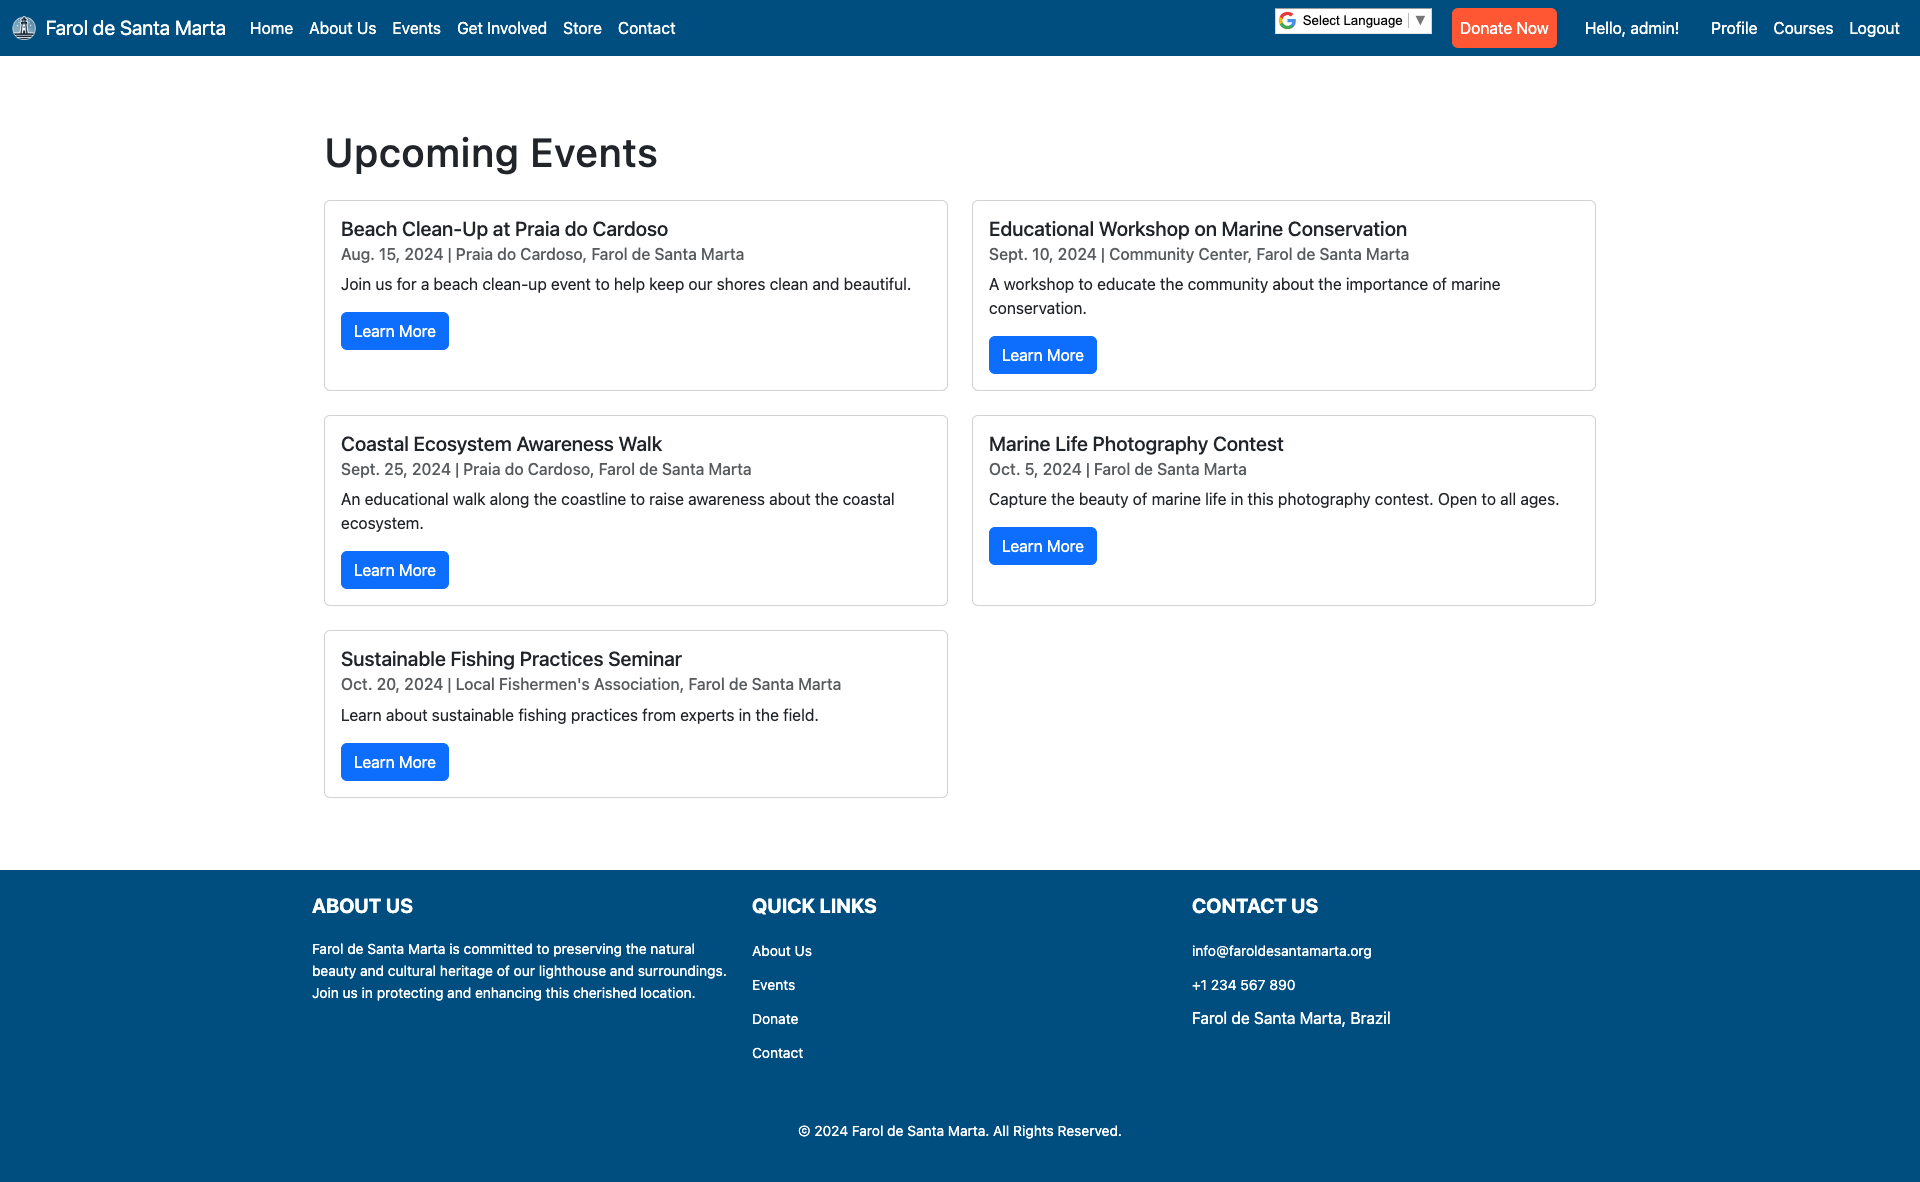
\includegraphics[width=\textwidth]{images/events-page.png}
    \caption{Example of the Events Page}
    \label{fig:events_page}
\end{figure}

\subsection{Donate Page}

The \textbf{Donate Page} is designed to facilitate financial contributions to support the ongoing conservation initiatives of \textit{Farol de Santa Marta}. The page offers a streamlined donation process, allowing users to select a predefined amount or enter a custom donation. Secure payment processing is integrated, ensuring that contributions are handled safely. The page also provides information on how donations are used, reinforcing transparency and encouraging user trust and generosity.

\begin{figure}[H]
    \centering
    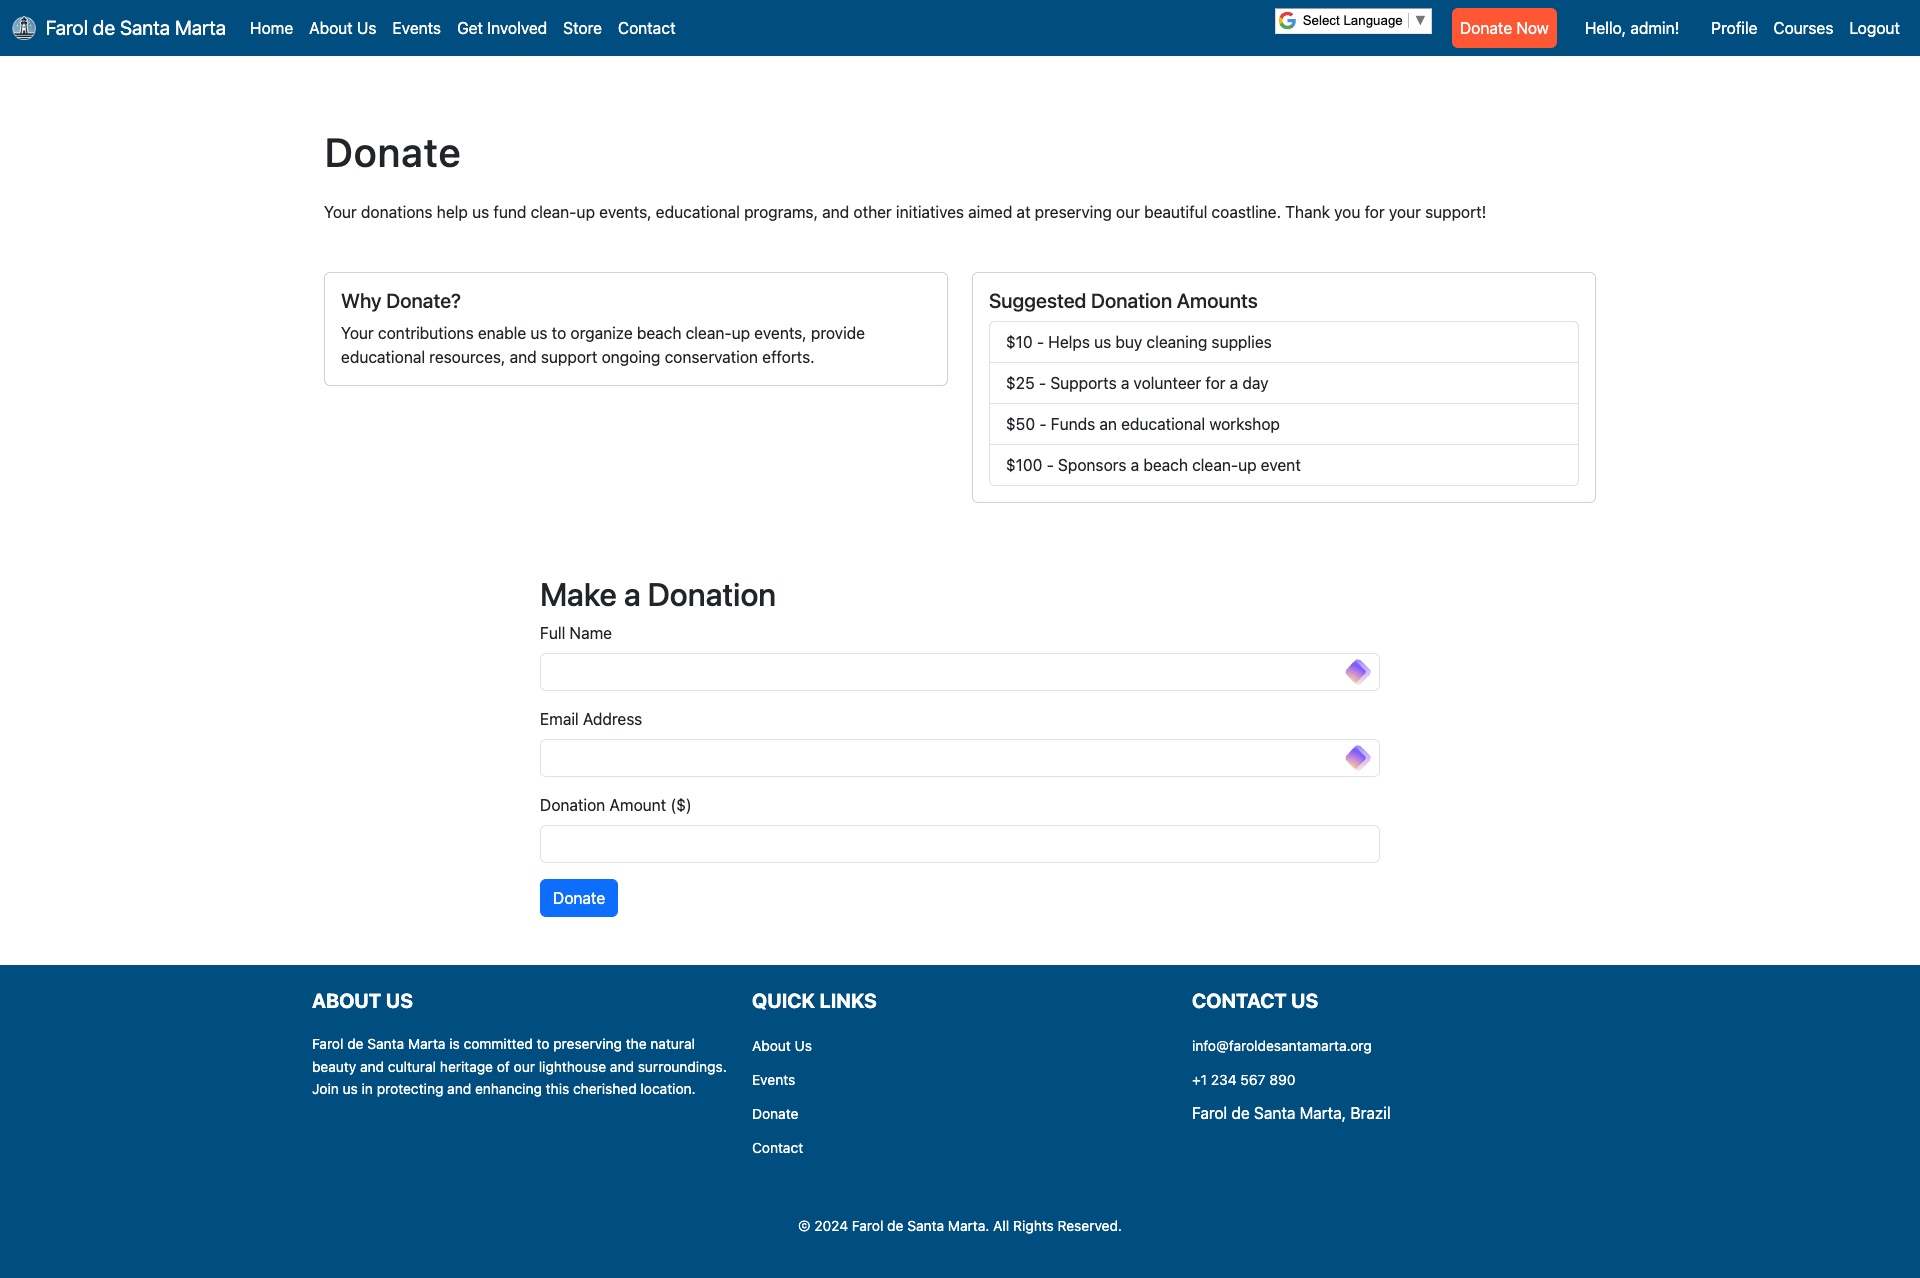
\includegraphics[width=\textwidth]{images/donate-page.png}
    \caption{Example of the Donate Page}
    \label{fig:donate_page}
\end{figure}

\subsection{Store Page}

The \textbf{Store Page} offers users the opportunity to purchase eco-friendly products, with all proceeds supporting the environmental initiatives of the organization. The store features items such as reusable water bottles, tote bags, and other sustainable goods, each accompanied by a description, price, and product image. This page not only serves as a fundraising tool but also promotes sustainable living by offering environmentally responsible products.

\begin{figure}[H]
    \centering
    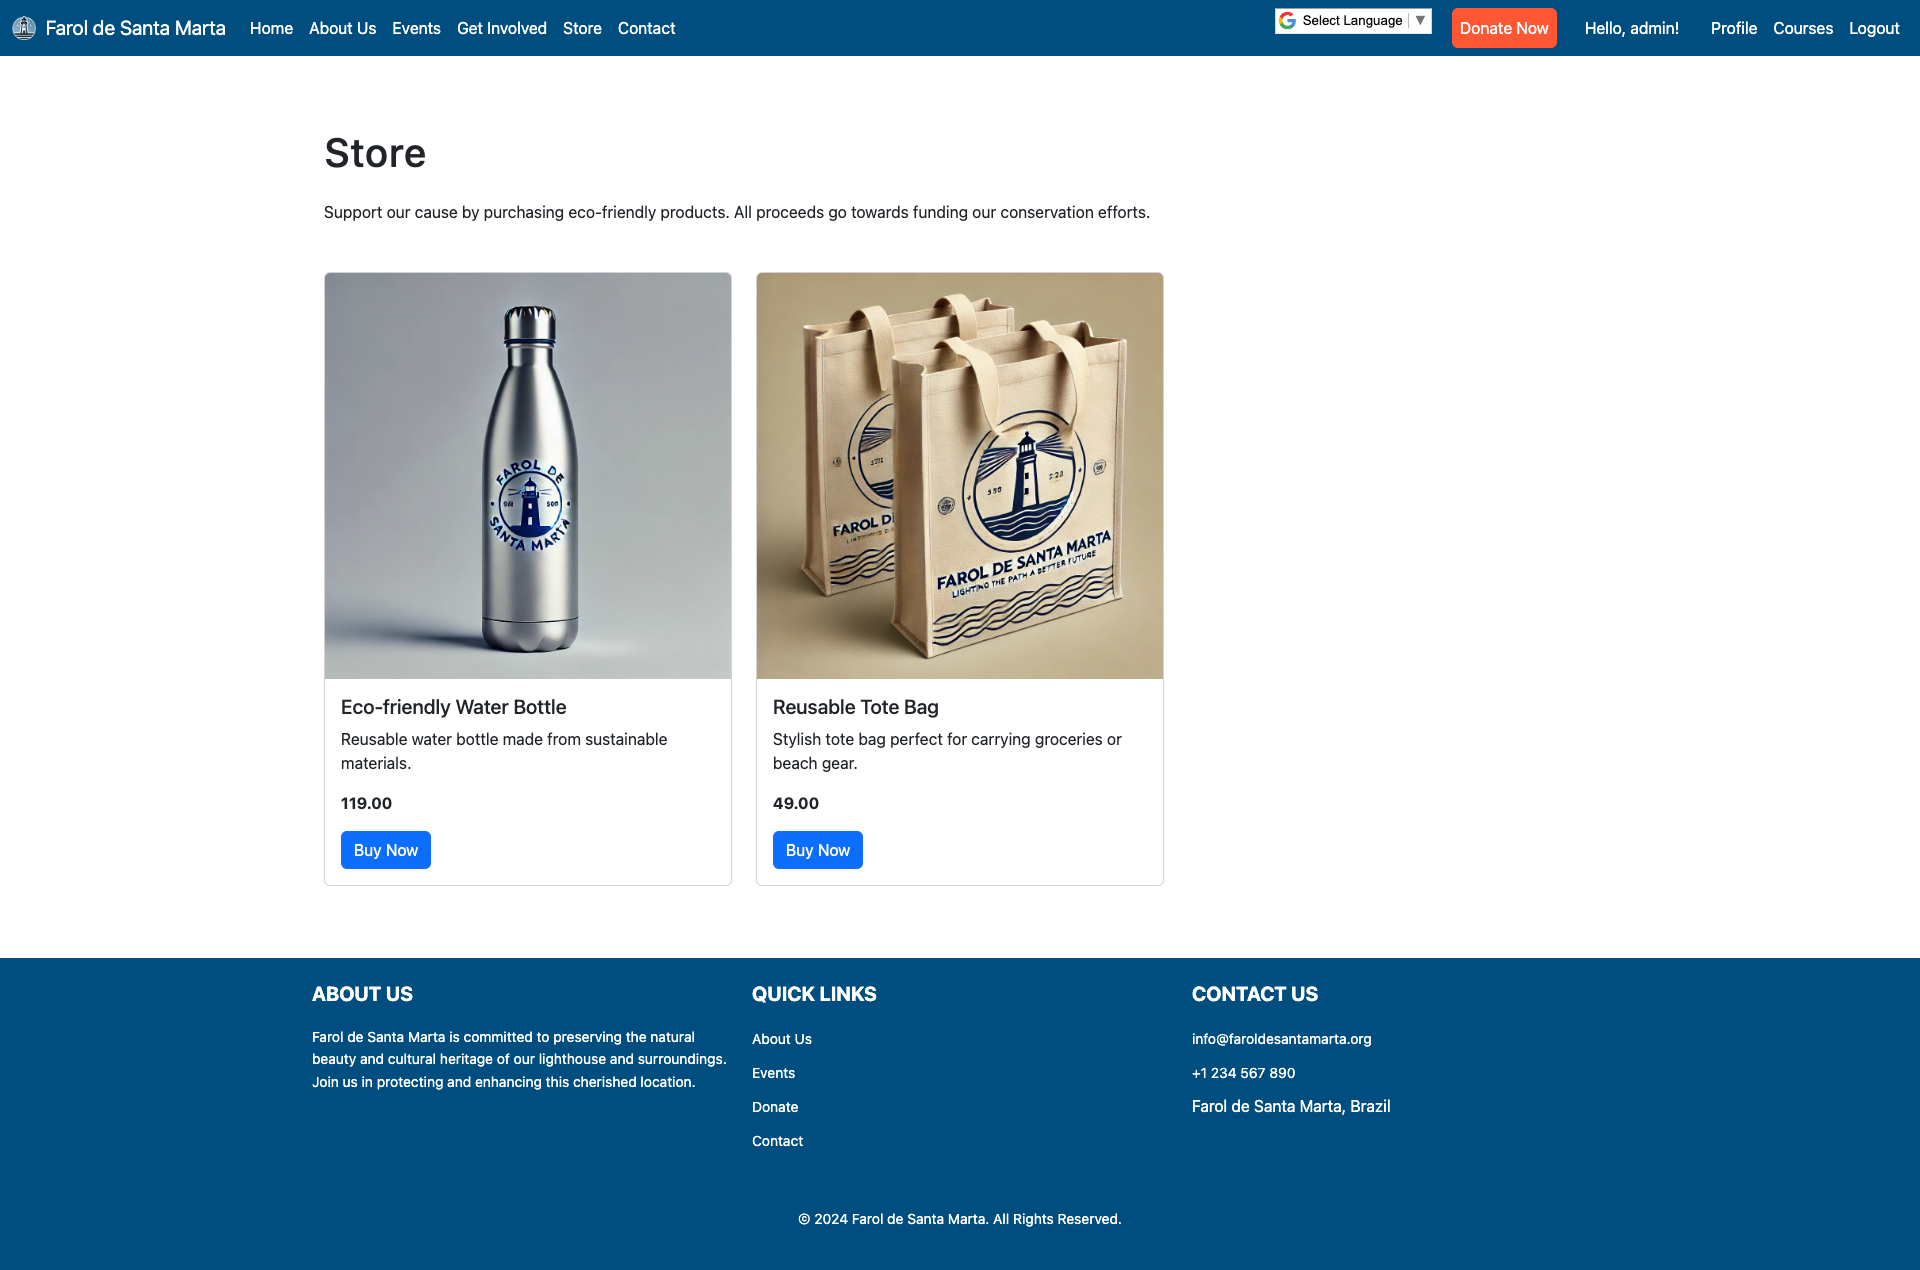
\includegraphics[width=\textwidth]{images/store-page.png}
    \caption{Example of the Store Page}
    \label{fig:store_page}
\end{figure}

\subsection{Courses Page}

The \textbf{Courses Page} provides access to educational resources focused on environmental conservation. Users, particularly students, can browse and enroll in various courses designed to enhance their understanding of sustainable practices and local environmental issues. Each course listing includes a description, instructor information, and any associated materials, fostering a learning environment that supports the mission of \textit{Farol de Santa Marta}.

\begin{figure}[H]
    \centering
    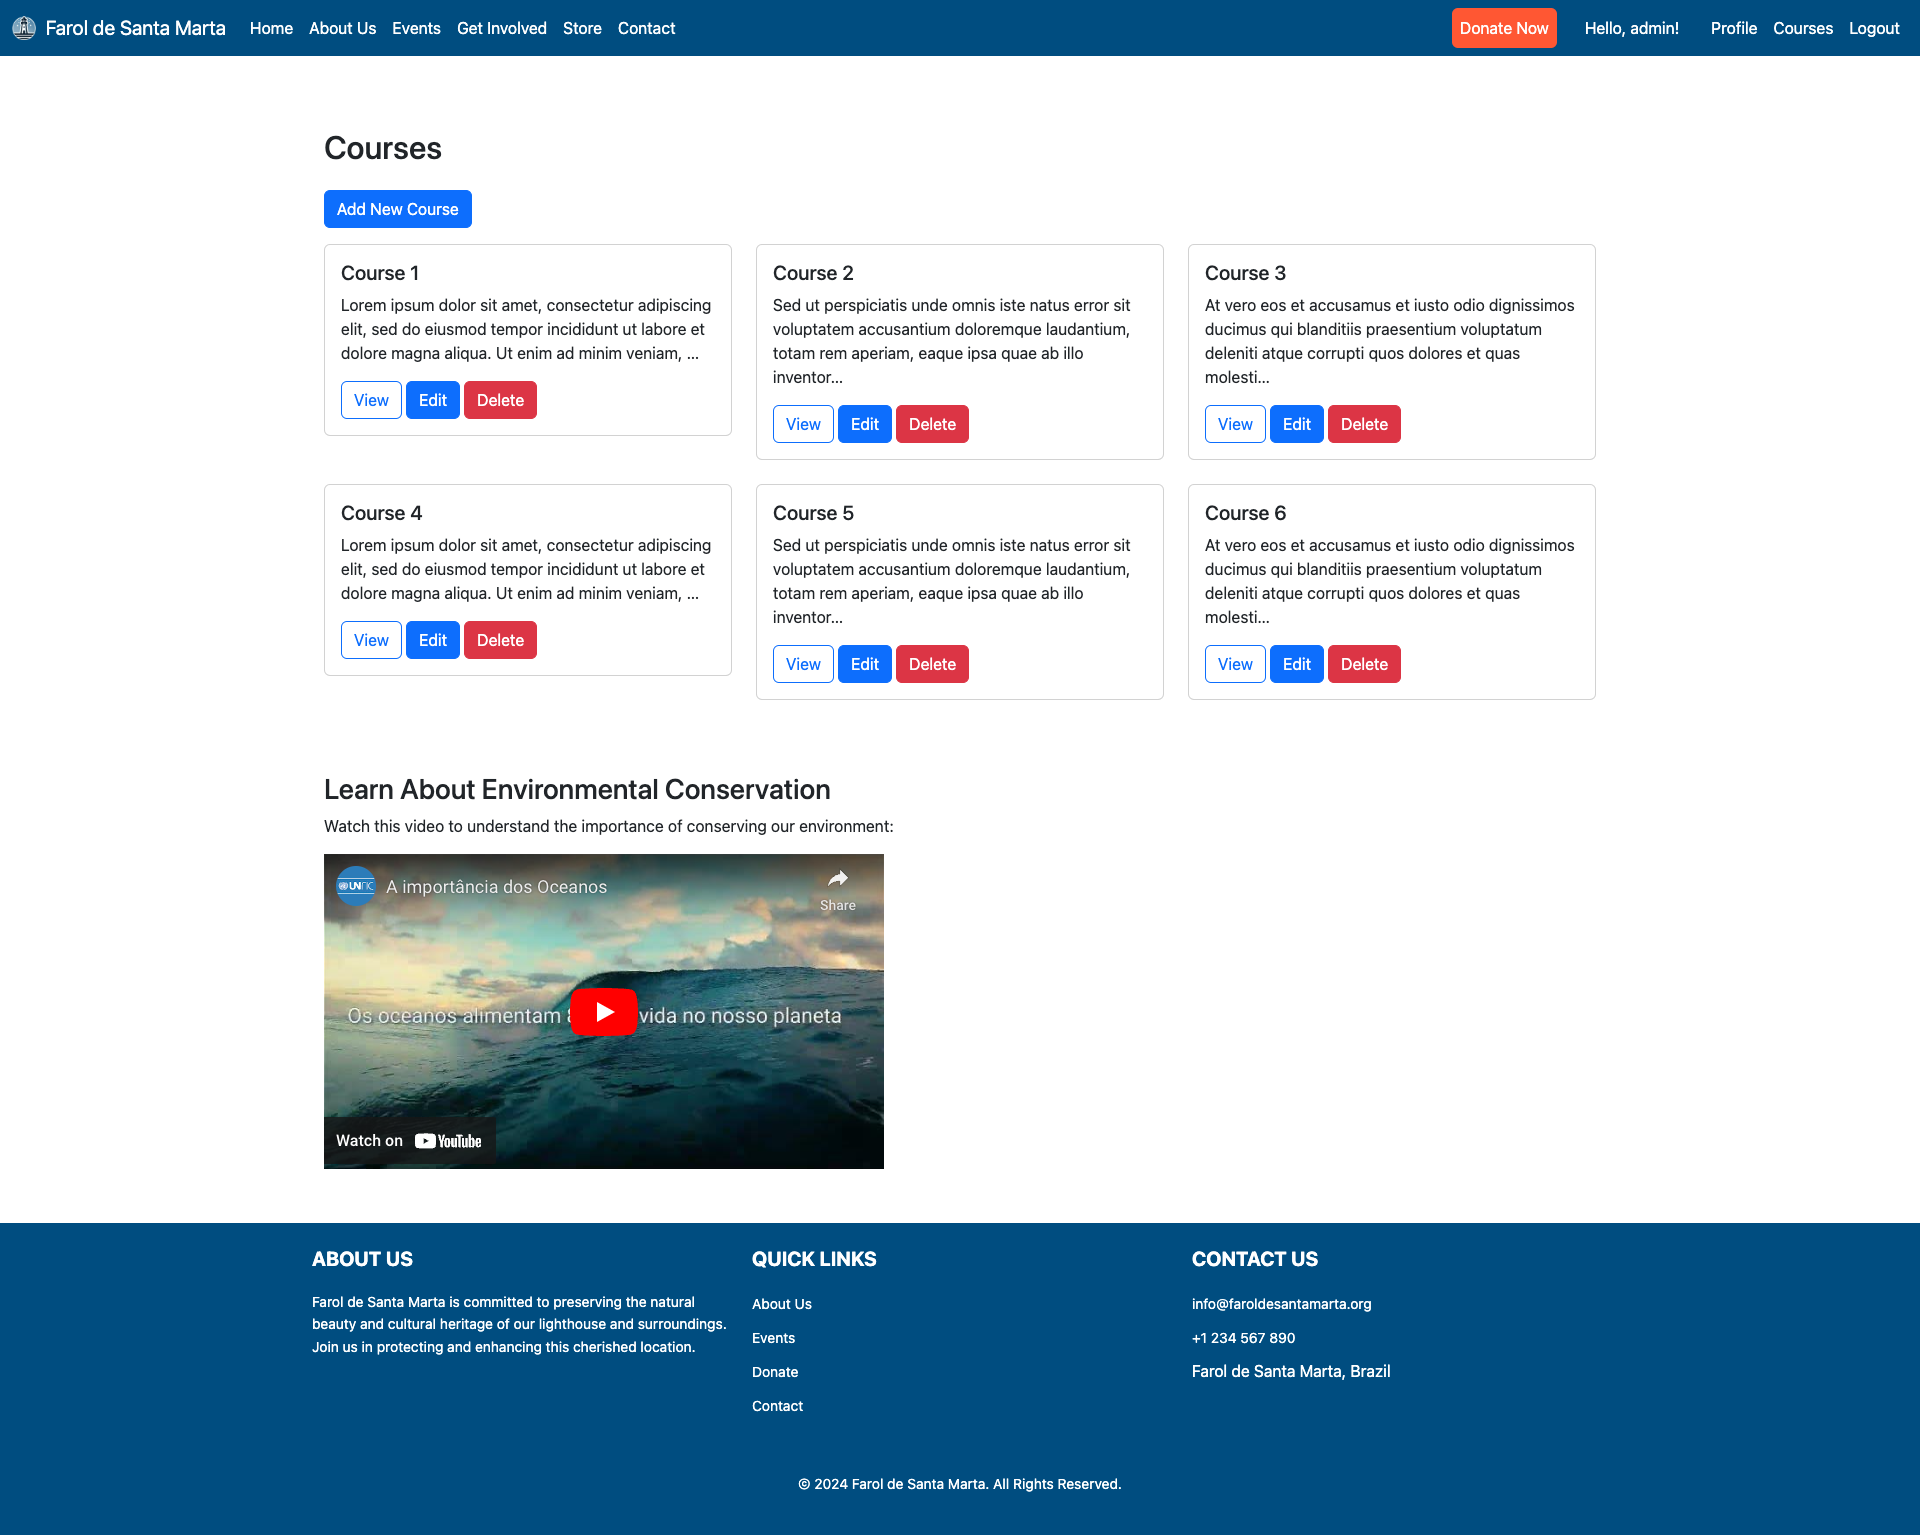
\includegraphics[width=\textwidth]{images/courses-page.png}
    \caption{Example of the Courses Page}
    \label{fig:courses_page}
\end{figure}

\subsection{Register Page}

The \textbf{Register Page} is the entry point for new users wishing to join the \textit{Farol de Santa Marta} community. It offers a straightforward registration process where users can create an account by providing essential information such as their name, email, and password. Upon successful registration, users gain access to additional features of the site, including event sign-ups, course enrollment, and the ability to make donations or purchases from the store.

\begin{figure}[H]
    \centering
    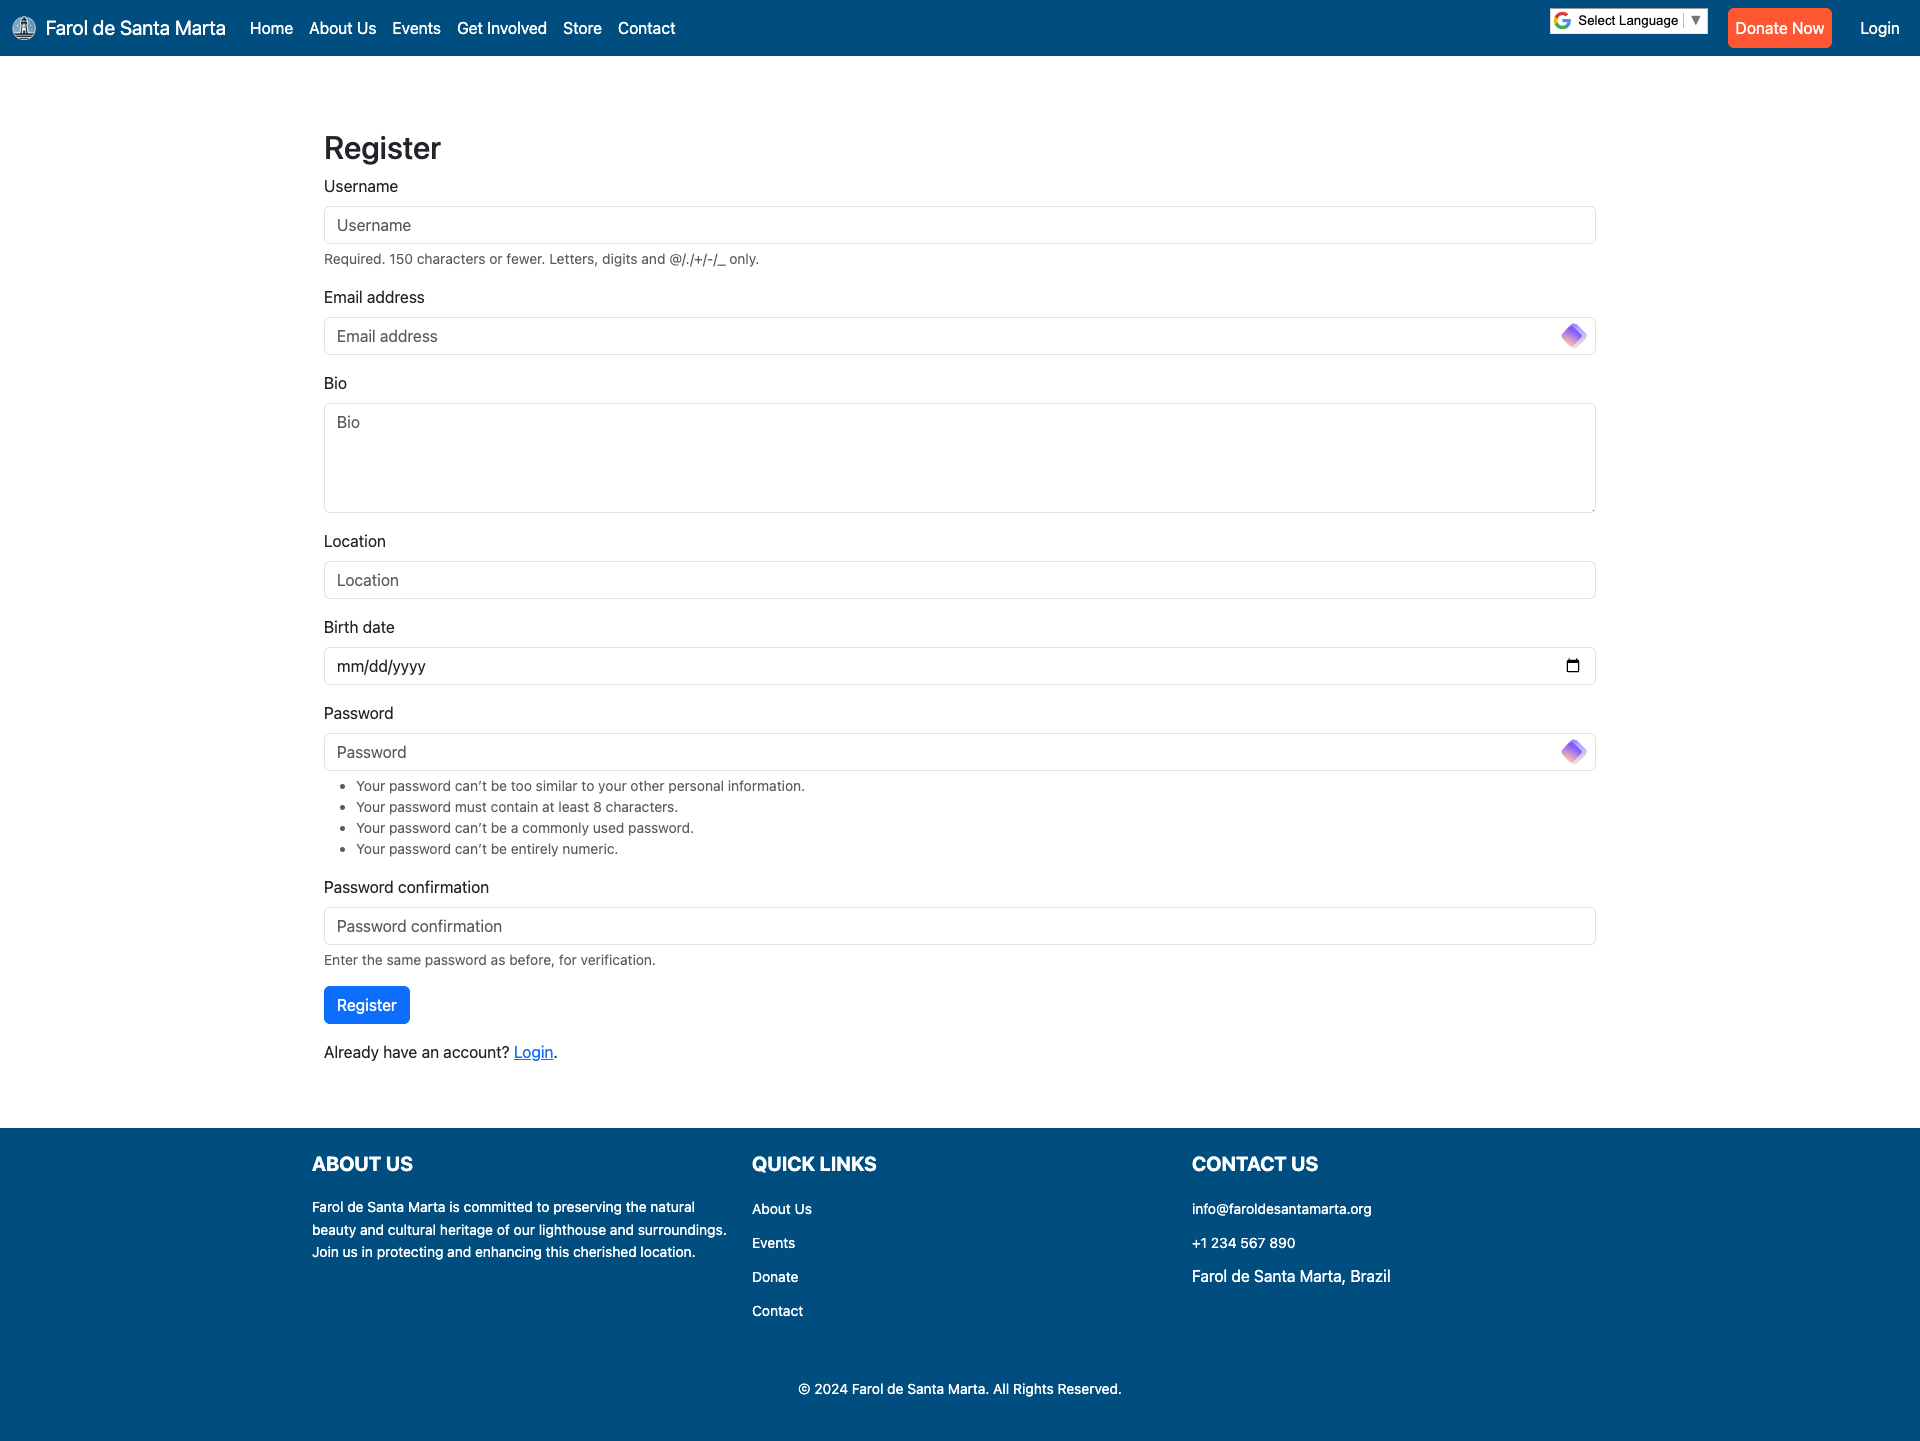
\includegraphics[width=\textwidth]{images/register-page.png}
    \caption{Example of the Register Page}
    \label{fig:register_page}
\end{figure}

\section{Technical Challenges}

During the development of the \textit{Farol de Santa Marta} website, several technical challenges were encountered, each requiring innovative solutions and persistent effort to overcome. This section discusses these challenges and the strategies employed to resolve them.

\subsection{Handling User Roles and Permissions}

Managing different user roles (e.g., students, teachers, and administrators) and their respective permissions presented a complex challenge, particularly in ensuring that each role had access only to the appropriate sections of the website.

This challenge was addressed by utilizing Django’s built-in user authentication and authorization system. Custom middleware was developed to enforce role-based access control, ensuring that users could only access pages and perform actions appropriate to their roles. Additionally, extensive testing was conducted to verify that the role-based permissions were correctly enforced across all features of the website.

\subsection{Database Design and Optimization}

Designing a robust database schema that could efficiently handle user data, course information, event details, and transaction records was a non-trivial task. The database needed to be optimized for performance while maintaining data integrity.

SQLite was selected as the database due to its simplicity and ease of integration with Django. The database schema was carefully designed to minimize redundancy and ensure efficient query performance. Indexing was implemented where necessary to speed up data retrieval, and Django’s ORM was used to manage database interactions securely and efficiently.

\section{GitHub Logs}

The GitHub logs provide a detailed record of all commits, showcasing the progress of the project from initial setup to final deployment. These logs are essential for understanding the development timeline and identifying significant milestones.

\begin{figure}[H]
    \centering
    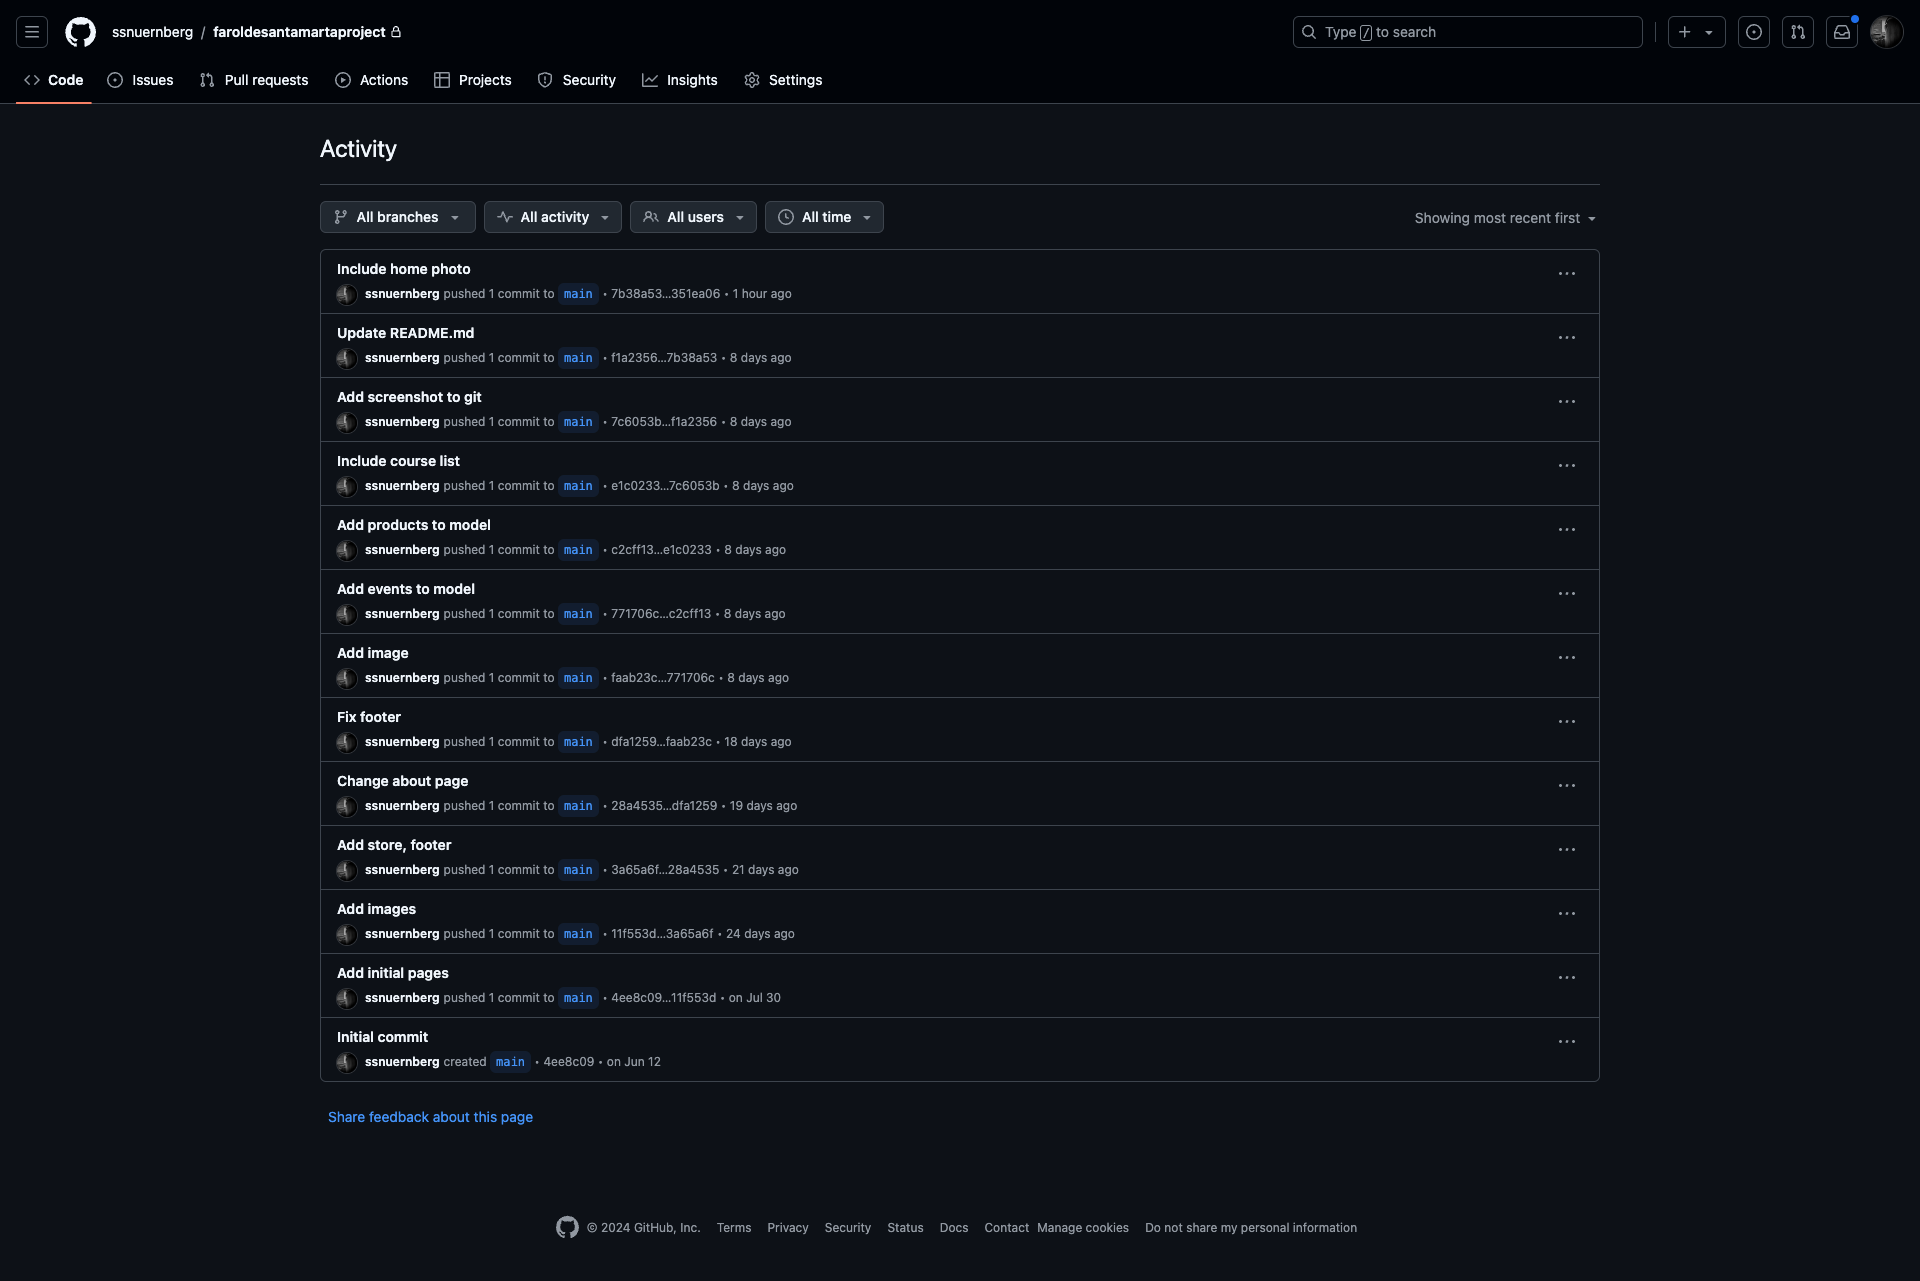
\includegraphics[width=\textwidth]{images/github-log.png}
    \caption{GitHub Logs of the \textit{Farol de Santa Marta} Project}
    \label{fig:github_logs}
\end{figure}

The logs illustrate the iterative nature of the development process. Key features such as user authentication, course management, and the donation system were developed incrementally, with regular commits ensuring that the project remained on track and aligned with the goals set out in the project plan.

The image in Figure \ref{fig:github_logs} provides a visual representation of the commit history, reflecting the steady progress and active development that characterized the \textit{Farol de Santa Marta} project.

The project will be public for access when published at \url{https://github.com/ssnuernberg/faroldesantamartaproject} and \url{http://www.faroldesantamarta.org}.



%%% Local Variables:
%%% mode: latex
%%% TeX-master: "../../main"
%%% End: